% Multiple Choice Question 8

\begin{center}
    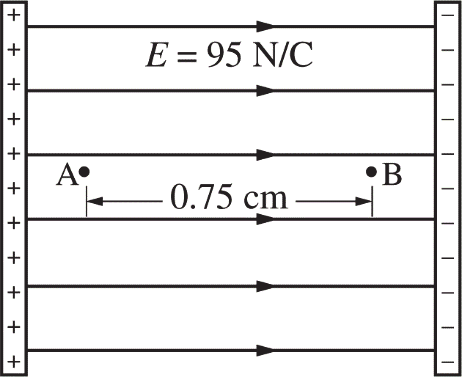
\includegraphics[scale=0.3]{images/img-005-005.png}
\end{center}

\begin{questions}
\setcounter{question}{7}

\question
Two conducting plates hold equal and opposite charges that create an electric field of magnitude $E = 95 \unit{N/C}$ that is directed to the right, as shown in the figure above. Points $\mathrm{A}$ and $\mathrm{B}$ are $0.75 \unit{cm}$ apart with $\mathrm{A}$ closer to the positive plate. A proton is released from rest at point $A$. What is the kinetic energy of the proton when it reaches point B?

\begin{choices}
    \choice $0$
    \choice $+1.14 \times 10^{-19} \unit{J}$
    \choice $+1.52 \times 10^{-17} \unit{J}$
    \choice $+1.92 \times 10^{-7} \unit{J}$
    \choice $+71 \unit{J}$
\end{choices}

\end{questions}
